\chapter{Flattened lightcurves and Periodograms of archival observations}
\label{archive_obs}


\begin{figure}
 \centering
 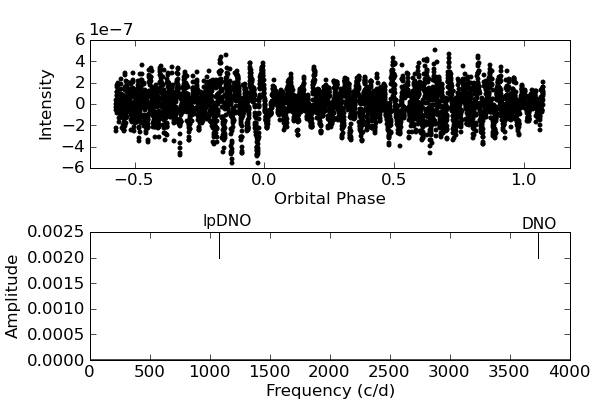
\includegraphics[bb=0 0 600 400,width=0.85\columnwidth]{images/archive_phot/S6544/S6544_c_FF.png}
 % S6544_c_FF.png: 600x400 pixel, 100dpi, 15.24x10.16 cm, bb=0 0 432 288
 \caption{S6544 Filtered lightcurve and periodogram}
 \label{S6544_c_FF}
\end{figure}


\begin{figure}
 \centering
 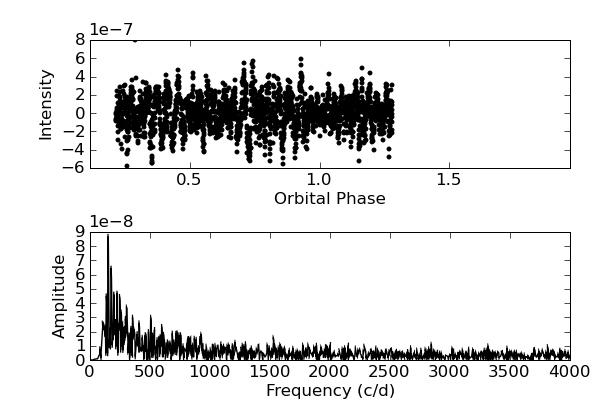
\includegraphics[bb=0 0 600 400,width=0.85\columnwidth]{images/archive_phot/S6548/S6548d_c_FF.png}
 % S6544_c_FF.png: 600x400 pixel, 100dpi, 15.24x10.16 cm, bb=0 0 432 288
 \caption{S6548 Filtered lightcurve and periodogram}
 \label{S6548_c_FF}
\end{figure}


\begin{figure}
 \centering
 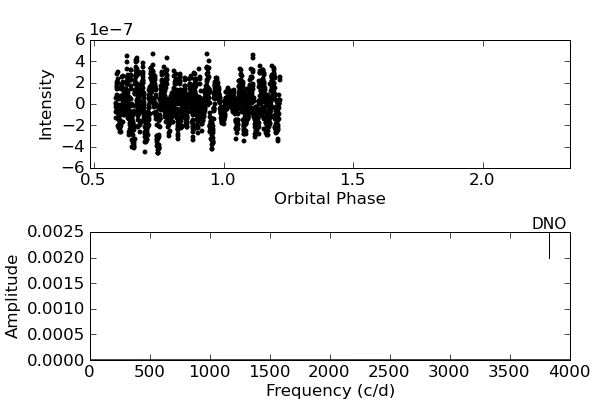
\includegraphics[bb=0 0 600 400,width=0.85\columnwidth]{images/archive_phot/S6549/S6549d_FF.png}
 % S6544_c_FF.png: 600x400 pixel, 100dpi, 15.24x10.16 cm, bb=0 0 432 288
 \caption{S6549 Filtered lightcurve and periodogram}
 \label{S6549_c_FF}
\end{figure}

\begin{figure}
 \centering
 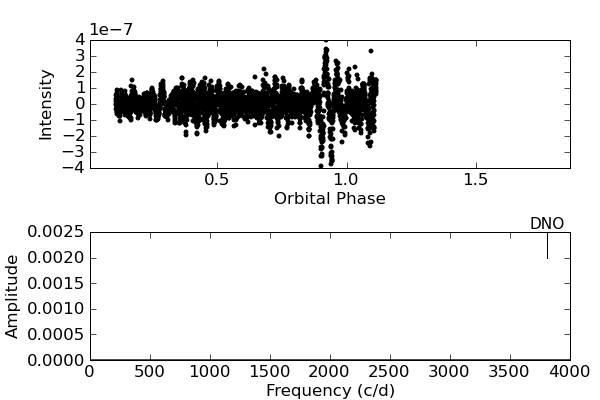
\includegraphics[bb=0 0 600 400,width=0.85\columnwidth]{images/archive_phot/S6551/S6551d_FF.png}
 % S6544_c_FF.png: 600x400 pixel, 100dpi, 15.24x10.16 cm, bb=0 0 432 288
 \caption{S6551 Filtered lightcurve and periodogram}
 \label{S6551_c_FF}
\end{figure}



\begin{figure}
 \centering
 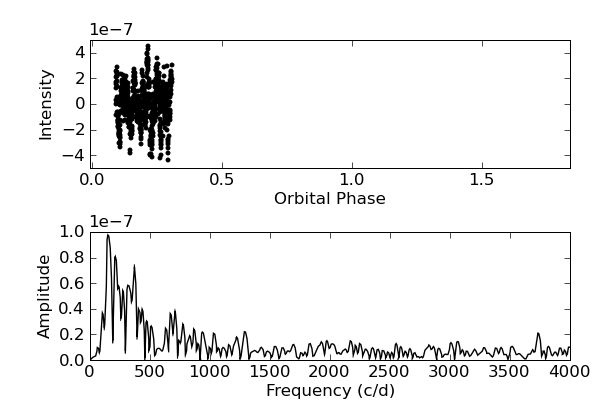
\includegraphics[bb=0 0 600 400,width=0.85\columnwidth]{images/archive_phot/S6553/S6553d_FF.png}
 % S6544_c_FF.png: 600x400 pixel, 100dpi, 15.24x10.16 cm, bb=0 0 432 288
 \caption{S6553 Filtered lightcurve and periodogram}
 \label{S6553_c_FF}
\end{figure}

\begin{figure}
 \centering
 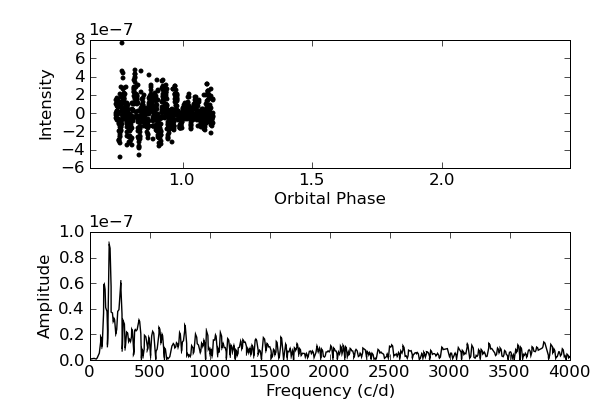
\includegraphics[bb=0 0 600 400,width=0.85\columnwidth]{images/archive_phot/S6555/S6555d_FF.png}
 % S6544_c_FF.png: 600x400 pixel, 100dpi, 15.24x10.16 cm, bb=0 0 432 288
 \caption{S6555 Filtered lightcurve and periodogram}
 \label{S6555_c_FF}
\end{figure}

\begin{figure}
 \centering
 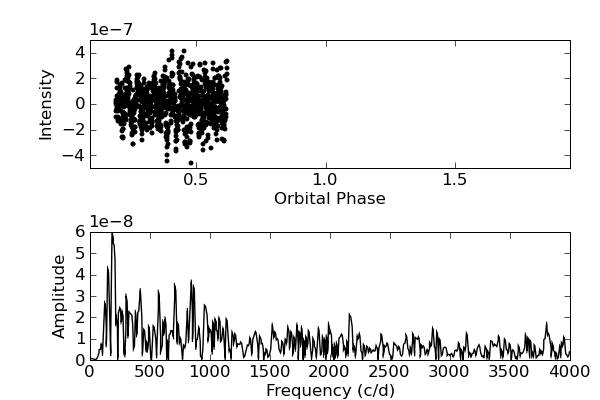
\includegraphics[bb=0 0 600 400,width=0.85\columnwidth]{images/archive_phot/S6557/S6557d_FF.png}
 % S6544_c_FF.png: 600x400 pixel, 100dpi, 15.24x10.16 cm, bb=0 0 432 288
 \caption{S6557 Filtered lightcurve and periodogram}
 \label{S6557_c_FF}
\end{figure}

\begin{figure}
 \centering
 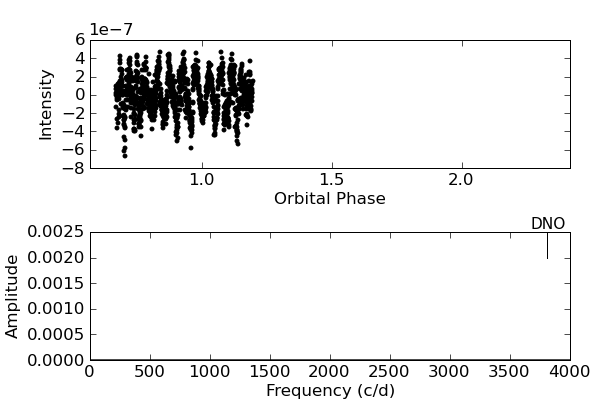
\includegraphics[bb=0 0 600 400,width=0.85\columnwidth]{images/archive_phot/S6564/S6564d_FF.png}
 % S6544_c_FF.png: 600x400 pixel, 100dpi, 15.24x10.16 cm, bb=0 0 432 288
 \caption{S6564 Filtered lightcurve and periodogram}
 \label{S6564_c_FF}
\end{figure}

\begin{figure}
 \centering
 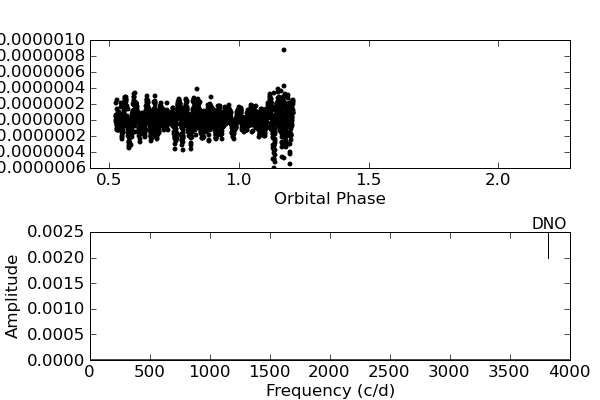
\includegraphics[bb=0 0 600 400,width=0.85\columnwidth]{images/archive_phot/S6570/S6570d_FF.png}
 % S6544_c_FF.png: 600x400 pixel, 100dpi, 15.24x10.16 cm, bb=0 0 432 288
 \caption{S6570 Filtered lightcurve and periodogram}
 \label{S6570_c_FF}
\end{figure}

\begin{figure}
 \centering
 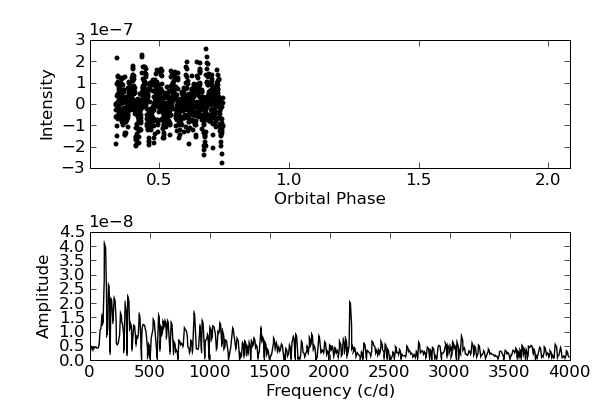
\includegraphics[bb=0 0 600 400,width=0.85\columnwidth]{images/archive_phot/S6574/S6574d_FF.png}
 % S6544_c_FF.png: 600x400 pixel, 100dpi, 15.24x10.16 cm, bb=0 0 432 288
 \caption{S6574 Filtered lightcurve and periodogram}
 \label{S6574_c_FF}
\end{figure}

\begin{figure}
 \centering
 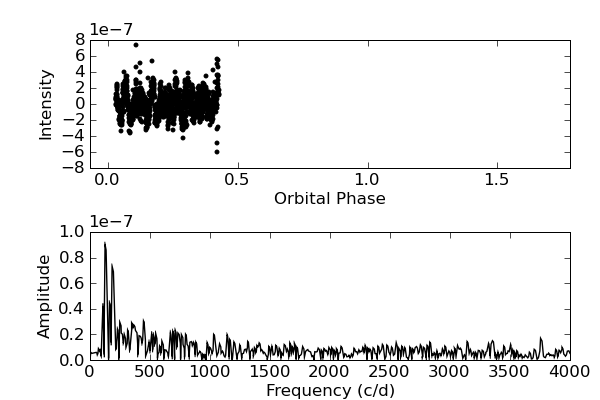
\includegraphics[bb=0 0 600 400,width=0.85\columnwidth]{images/archive_phot/S6580/S6580d_FF.png}
 % S6544_c_FF.png: 600x400 pixel, 100dpi, 15.24x10.16 cm, bb=0 0 432 288
 \caption{S6580 Filtered lightcurve and periodogram}
 \label{S6580_c_FF}
\end{figure}

\begin{figure}
 \centering
 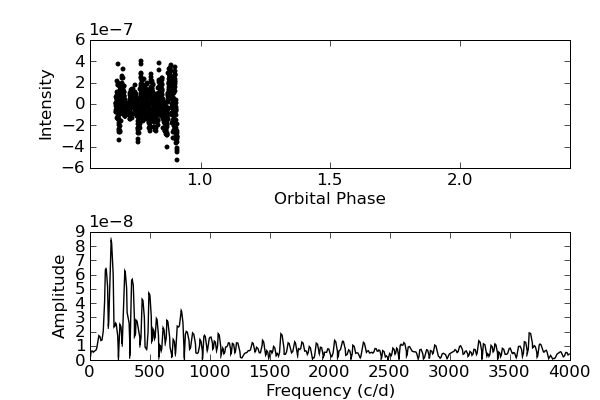
\includegraphics[bb=0 0 600 400,width=0.85\columnwidth]{images/archive_phot/S6599/S6599d_FF.png}
 % S6544_c_FF.png: 600x400 pixel, 100dpi, 15.24x10.16 cm, bb=0 0 432 288
 \caption{S6599 Filtered lightcurve and periodogram}
 \label{S6599_c_FF}
\end{figure}

\begin{figure}
 \centering
 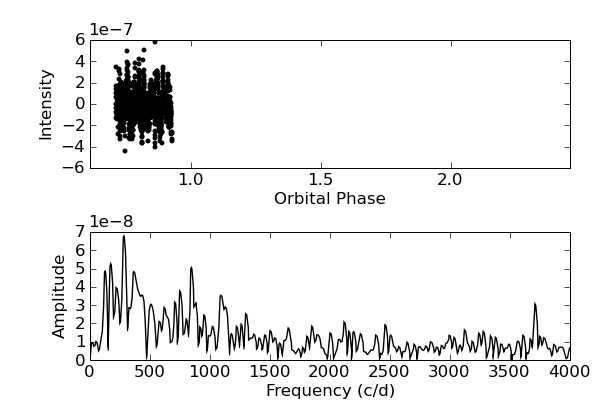
\includegraphics[bb=0 0 600 400,width=0.85\columnwidth]{images/archive_phot/S6634/S6634d_FF.png}
 % S6544_c_FF.png: 600x400 pixel, 100dpi, 15.24x10.16 cm, bb=0 0 432 288
 \caption{S6634 Filtered lightcurve and periodogram}
 \label{S6634_c_FF}
\end{figure}

\begin{figure}
 \centering
 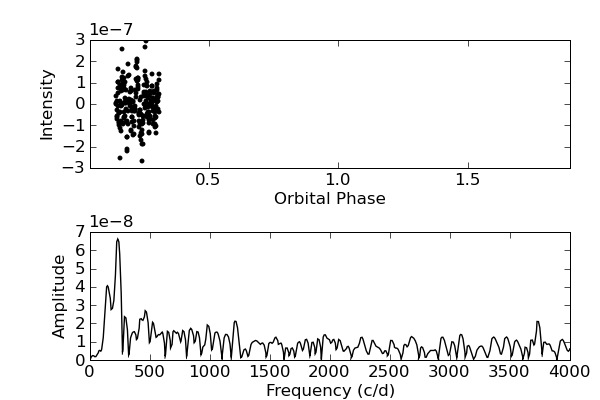
\includegraphics[bb=0 0 600 400,width=0.85\columnwidth]{images/archive_phot/S6639/S6639d_FF.png}
 % S6544_c_FF.png: 600x400 pixel, 100dpi, 15.24x10.16 cm, bb=0 0 432 288
 \caption{S6639 Filtered lightcurve and periodogram}
 \label{S6639_c_FF}
\end{figure}

\begin{figure}
 \centering
 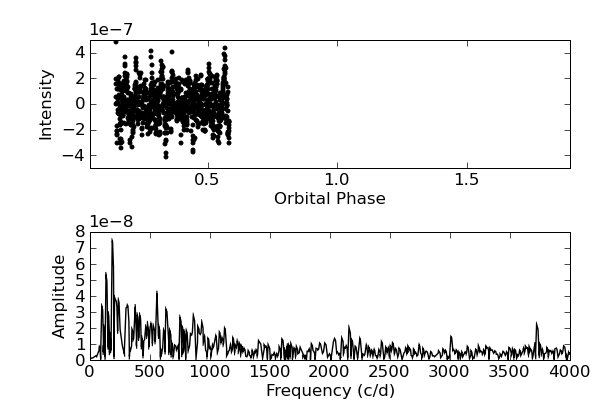
\includegraphics[bb=0 0 600 400,width=0.85\columnwidth]{images/archive_phot/S6641/S6641d_FF.png}
 % S6544_c_FF.png: 600x400 pixel, 100dpi, 15.24x10.16 cm, bb=0 0 432 288
 \caption{S6641 Filtered lightcurve and periodogram}
 \label{S6641_c_FF}
\end{figure}

\begin{figure}
 \centering
 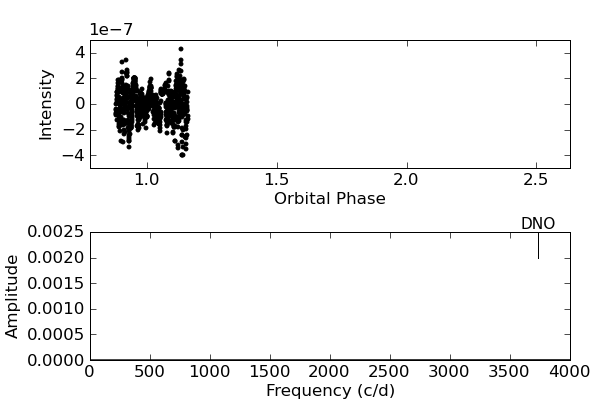
\includegraphics[bb=0 0 600 400,width=0.85\columnwidth]{images/archive_phot/S6660/S6660d_FF.png}
 % S6544_c_FF.png: 600x400 pixel, 100dpi, 15.24x10.16 cm, bb=0 0 432 288
 \caption{S6660 Filtered lightcurve and periodogram}
 \label{S6660_c_FF}
\end{figure}

\begin{figure}
 \centering
 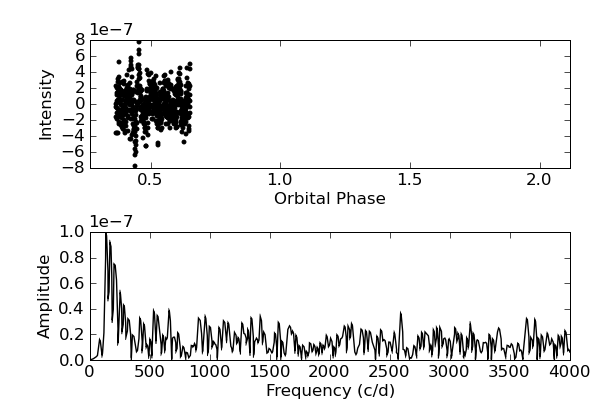
\includegraphics[bb=0 0 600 400,width=0.85\columnwidth]{images/archive_phot/S6666/S6666d_FF.png}
 % S6544_c_FF.png: 600x400 pixel, 100dpi, 15.24x10.16 cm, bb=0 0 432 288
 \caption{S6666 Filtered lightcurve and periodogram}
 \label{S6666_c_FF}
\end{figure}

\begin{figure}
 \centering
 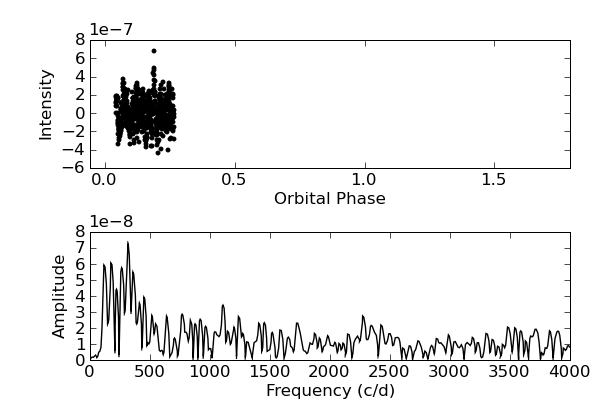
\includegraphics[bb=0 0 600 400,width=0.85\columnwidth]{images/archive_phot/S6670/S6670d_FF.png}
 % S6544_c_FF.png: 600x400 pixel, 100dpi, 15.24x10.16 cm, bb=0 0 432 288
 \caption{S6670 Filtered lightcurve and periodogram}
 \label{S6670_c_FF}
\end{figure}



\chapter{$O-C$ diagrams of archival observations}
\label{OminC_archive}
% add pagebreak to stop too many unprocessed floats error
%\pagebreak

\begin{figure}
 \centering
 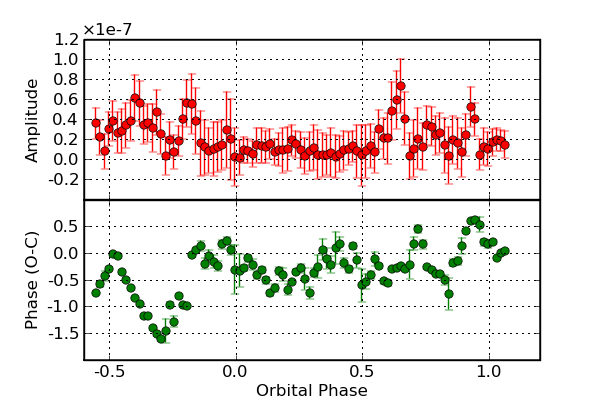
\includegraphics[bb=0 0 600 400,width=0.85\columnwidth]{images/archive_phot/S6544/S6544_23.13.png}
 % S6544_23.13.png: 600x400 pixel, 100dpi, 15.24x10.16 cm, bb=0 0 600 400
 \caption[S6544 $O-C$ diagram of DNO]{Amplitude and $O-C$ variation of 23.13 s DNO of run S6544. Diagrams were calculated relative to a period of 23.13 s using 20 cycles with 50\% overlap. }
 \label{S6544_23.13}
\end{figure}

\begin{figure}
 \centering
 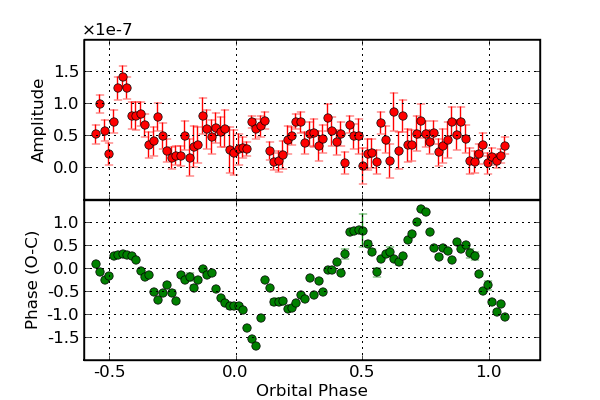
\includegraphics[bb=0 0 600 400,width=0.85\columnwidth]{images/archive_phot/S6544/S6544_94.26.png}
 % S6544_23.13.png: 600x400 pixel, 100dpi, 15.24x10.16 cm, bb=0 0 600 400
 \caption[S6544 $O-C$ diagram of lDNO]{Amplitude and $O-C$ variation of 94.26 s DNO of run S6544. Diagrams were calculated relative to a period of 94.26 s using 5 cycles with 50\% overlap. }
 \label{S6544_94.26}
\end{figure}

\begin{figure}
 \centering
 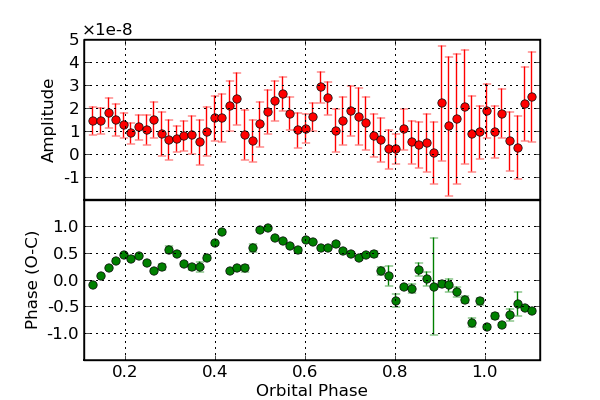
\includegraphics[bb=0 0 600 400,width=0.85\columnwidth]{images/archive_phot/S6551/S6551d_22.69.png}
 % S6544_23.13.png: 600x400 pixel, 100dpi, 15.24x10.16 cm, bb=0 0 600 400
 \caption[S6551 $O-C$ diagram of DNO]{Amplitude and $O-C$ variation of 22.69 s DNO of run S6551. Diagrams were calculated relative to a period of 22.69 s using 20 cycles with 50\% overlap. }
 \label{S6551_22.69}
\end{figure}


\begin{figure}
 \centering
 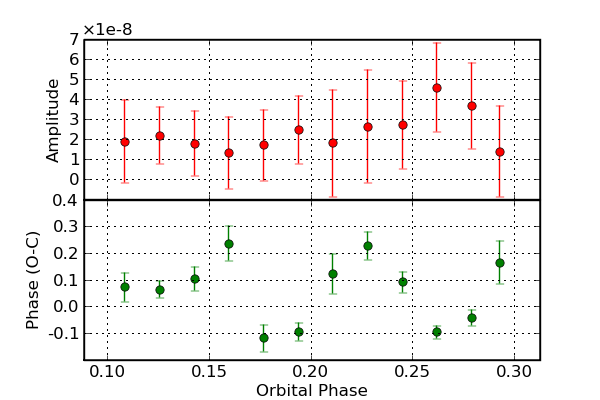
\includegraphics[bb=0 0 600 400,width=0.85\columnwidth]{images/archive_phot/S6553/S6553d_23.13.png}
 % S6544_23.13.png: 600x400 pixel, 100dpi, 15.24x10.16 cm, bb=0 0 600 400
 \caption[S6553 $O-C$ diagram of DNO]{Amplitude and $O-C$ variation of 23.13 s DNO of run S6553. Diagrams were calculated relative to a period of 23.13 s using 20 cycles with 50\% overlap. }
 \label{S6553_23.13}
\end{figure}


\begin{figure}
 \centering
 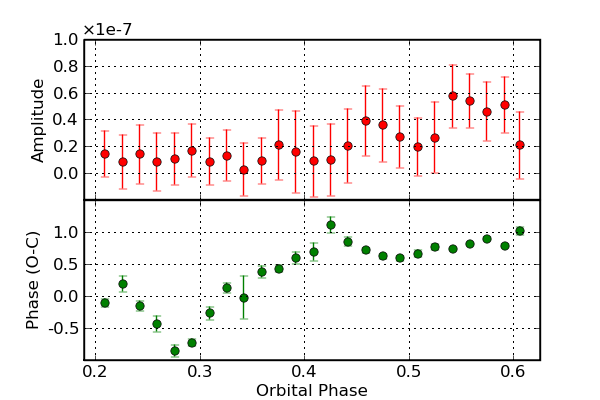
\includegraphics[bb=0 0 600 400,width=0.85\columnwidth]{images/archive_phot/S6557/S6557_22.72.png}
 % S6544_23.13.png: 600x400 pixel, 100dpi, 15.24x10.16 cm, bb=0 0 600 400
 \caption[S6557 $O-C$ diagram of DNO]{Amplitude and $O-C$ variation of 22.72 s DNO of run S6557. Diagrams were calculated relative to a period of 22.72 s using 20 cycles with 50\% overlap. }
 \label{S6557_22.72}
\end{figure}

% S6564
\begin{figure}
 \centering
 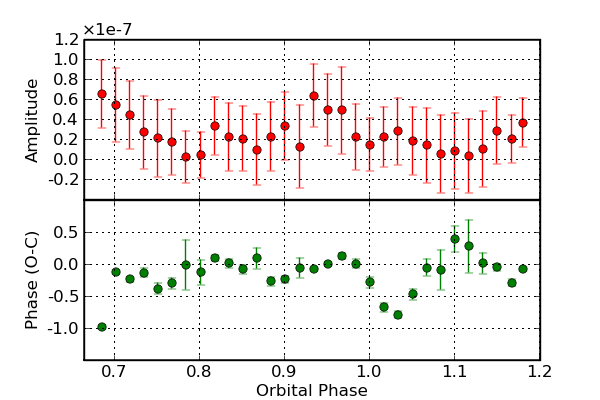
\includegraphics[bb=0 0 600 400,width=0.85\columnwidth]{images/archive_phot/S6564/S6564_22.68.png}
 % S6544_23.13.png: 600x400 pixel, 100dpi, 15.24x10.16 cm, bb=0 0 600 400
 \caption[S6564 $O-C$ diagram of DNO]{Amplitude and $O-C$ variation of 22.68 s DNO of run S6564. Diagrams were calculated relative to a period of 22.68 s using 20 cycles with 50\% overlap. The DNO's phase changes through $360^{\circ}$ during eclipse. }
 \label{S6564_22.68}
\end{figure}

% S6570
\begin{figure}
 \centering
 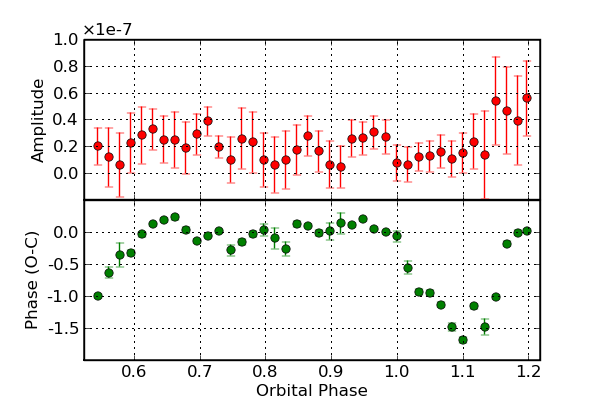
\includegraphics[bb=0 0 600 400,width=0.85\columnwidth]{images/archive_phot/S6570/S6570_22.63.png}
 % S6544_23.13.png: 600x400 pixel, 100dpi, 15.24x10.16 cm, bb=0 0 600 400
 \caption[S6570 $O-C$ diagram of DNO]{Amplitude and $O-C$ variation of 22.63 s DNO of run S6570. Diagrams were calculated relative to a period of 22.63 s using 20 cycles with 50\% overlap. The DNO's phase changes through $360^{\circ}$ during eclipse. }
 \label{S6570_22.63}
\end{figure}

% S6574
\begin{figure}
 \centering
 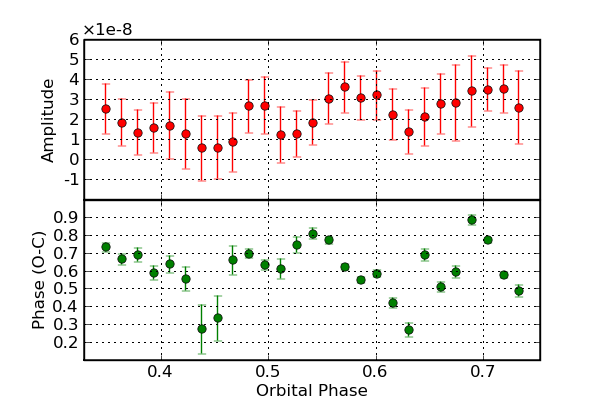
\includegraphics[bb=0 0 600 400,width=0.85\columnwidth]{images/archive_phot/S6574/S6574_39.85.png}
 % S6544_23.13.png: 600x400 pixel, 100dpi, 15.24x10.16 cm, bb=0 0 600 400
 \caption[S6574 $O-C$ diagram of 39.85 s DNO]{Amplitude and $O-C$ variation of 39.85 s DNO?of run S6574. Diagrams were calculated relative to a period of 39.85 s using 10 cycles with 50\% overlap. }
 \label{S6574_39.85}
\end{figure}

% S6599
\begin{figure}
 \centering
 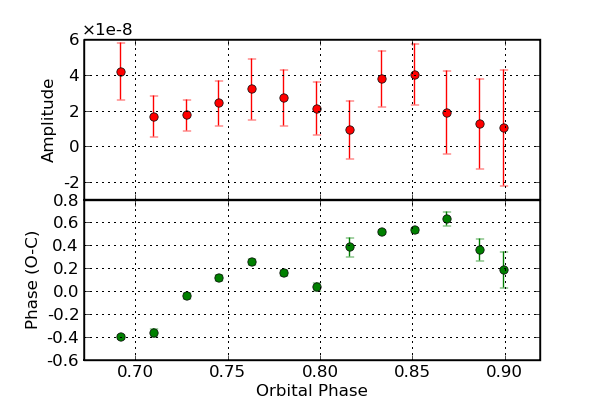
\includegraphics[bb=0 0 600 400,width=0.85\columnwidth]{images/archive_phot/S6599/S6599_23.56.png}
 % S6544_23.13.png: 600x400 pixel, 100dpi, 15.24x10.16 cm, bb=0 0 600 400
 \caption[S6599 $O-C$ diagram of 23.56 s DNO]{Amplitude and $O-C$ variation of 23.56 s DNO of run S6599. Diagrams were calculated relative to a period of 23.56 s using 20 cycles with 50\% overlap. }
 \label{S6599_23.56}
\end{figure}

% S6634
\begin{figure}
 \centering
 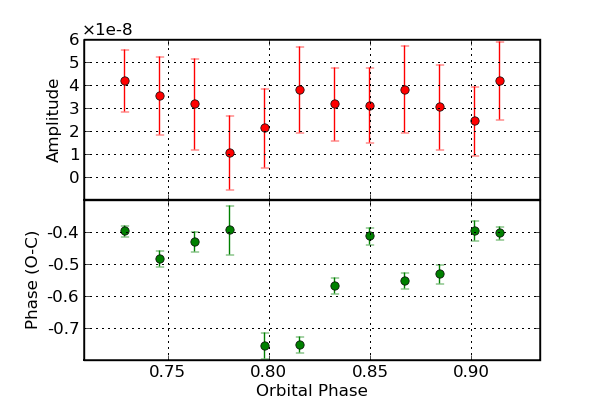
\includegraphics[bb=0 0 600 400,width=0.85\columnwidth]{images/archive_phot/S6634/S6634d_23.28.png}
 % S6544_23.13.png: 600x400 pixel, 100dpi, 15.24x10.16 cm, bb=0 0 600 400
 \caption[S6634 $O-C$ diagram of 23.28 s DNO]{Amplitude and $O-C$ variation of 23.28 s DNO of run S6634. Diagrams were calculated relative to a period of 23.28 s using 20 cycles with 50\% overlap. }
 \label{S6634_23.28}
\end{figure}

\begin{figure}
 \centering
 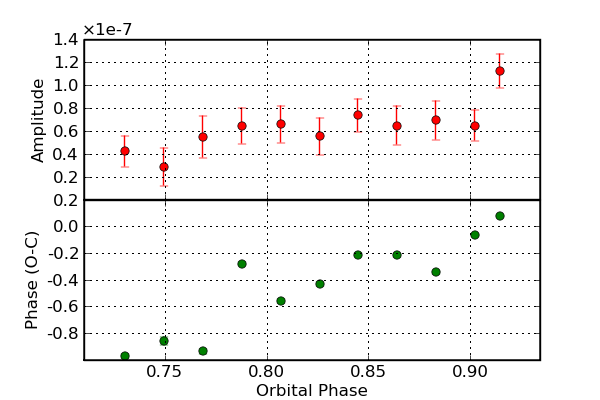
\includegraphics[bb=0 0 600 400,width=0.85\columnwidth]{images/archive_phot/S6634/S6634d_102.08.png}
 % S6544_23.13.png: 600x400 pixel, 100dpi, 15.24x10.16 cm, bb=0 0 600 400
 \caption[S6634 $O-C$ diagram of 102.08 s lpDNO]{Amplitude and $O-C$ variation of 102.08 s lpDNO of run S6634. Diagrams were calculated relative to a period of 102.08 s using 10 cycles with 50\% overlap. }
 \label{S6634_102.08}
\end{figure}

\begin{figure}
 \centering
 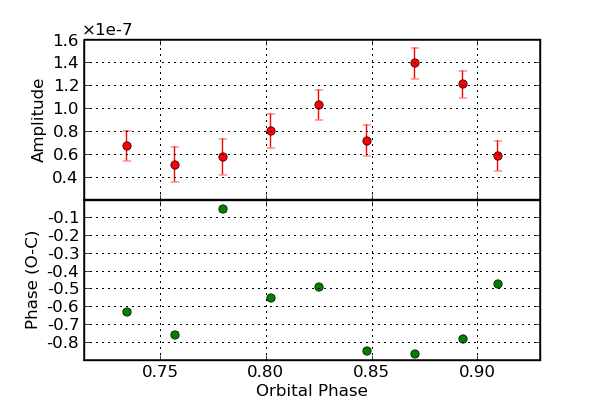
\includegraphics[bb=0 0 600 400,width=0.85\columnwidth]{images/archive_phot/S6634/S6634d_305.23.png}
 % S6544_23.13.png: 600x400 pixel, 100dpi, 15.24x10.16 cm, bb=0 0 600 400
 \caption[S6634 $O-C$ diagram of 305.23 s QPO]{Amplitude and $O-C$ variation of 305.23 s QPO of run S6634. Diagrams were calculated relative to a period of 305.23 s using 2 cycles with 50\% overlap. }
 \label{S6634_305.23}
\end{figure}


% S6639

\begin{figure}
 \centering
 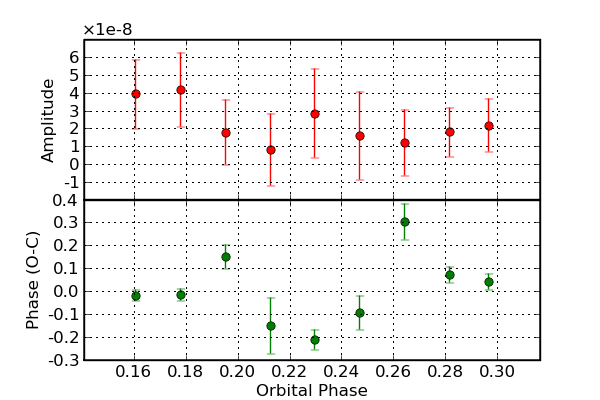
\includegraphics[bb=0 0 600 400,width=0.85\columnwidth]{images/archive_phot/S6639/S6639d_23.15.png}
 % S6544_23.13.png: 600x400 pixel, 100dpi, 15.24x10.16 cm, bb=0 0 600 400
 \caption[S6639 $O-C$ diagram of 23.15 s DNO]{Amplitude and $O-C$ variation of 23.15 s DNO of run S6639. Diagrams were calculated relative to a period of 23.15 s using 20 cycles with 50\% overlap. }
 \label{S6639_23.15}
\end{figure}


% S6641

\begin{figure}
 \centering
 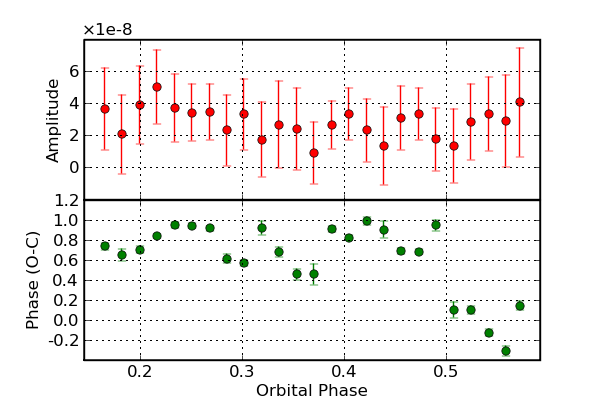
\includegraphics[bb=0 0 600 400,width=0.85\columnwidth]{images/archive_phot/S6641/S6641d_23.19.png}
 % S6544_23.13.png: 600x400 pixel, 100dpi, 15.24x10.16 cm, bb=0 0 600 400
 \caption[S6641 $O-C$ diagram of 23.19 s DNO]{Amplitude and $O-C$ variation of 23.19 s DNO of run S6641. Diagrams were calculated relative to a period of 23.19 s using 20 cycles with 50\% overlap. }
 \label{S6641_23.19}
\end{figure}


\begin{figure}
 \centering
 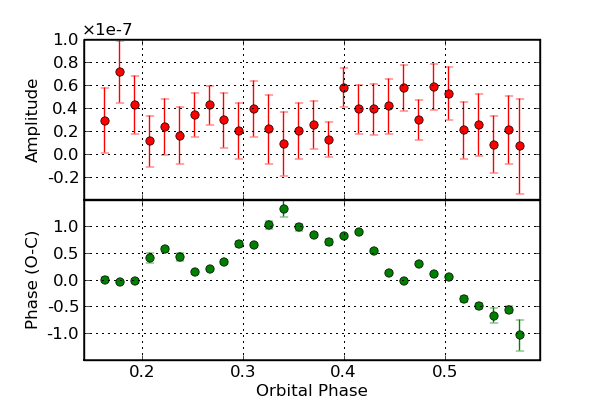
\includegraphics[bb=0 0 600 400,width=0.85\columnwidth]{images/archive_phot/S6641/S6641d_39.97.png}
 % S6544_23.13.png: 600x400 pixel, 100dpi, 15.24x10.16 cm, bb=0 0 600 400
 \caption[S6641 $O-C$ diagram of 39.97 s signal]{Amplitude and $O-C$ variation of 39.97 s signal of run S6641. Diagrams were calculated relative to a period of 39.97 s using 10 cycles with 50\% overlap. }
 \label{S6641_39.97}
\end{figure}


% S6660

\begin{figure}
 \centering
 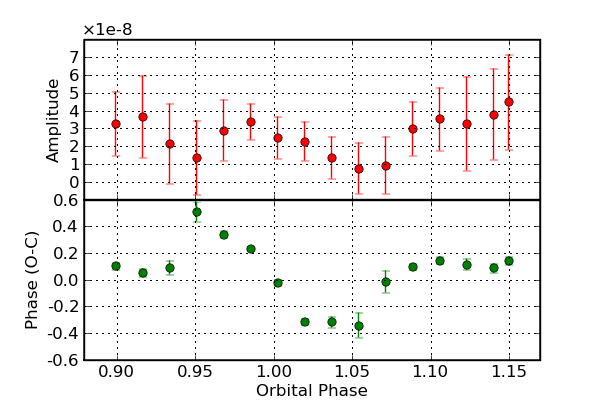
\includegraphics[bb=0 0 600 400,width=0.85\columnwidth]{images/archive_phot/S6660/SS6660d_23.16.fixed.png}
 % S6544_23.13.png: 600x400 pixel, 100dpi, 15.24x10.16 cm, bb=0 0 600 400
 \caption[S6660 $O-C$ diagram of 23.16 s DNO]{Amplitude and $O-C$ variation of 23.16 s DNO of run S6660. Diagrams were calculated relative to a period of 23.16 s using 20 cycles with 50\% overlap. The DNO undergoes a $360^{\circ}$ phase changes during eclipse.}
 \label{S6660_23.16}
\end{figure}


% S6670

\begin{figure}
 \centering
 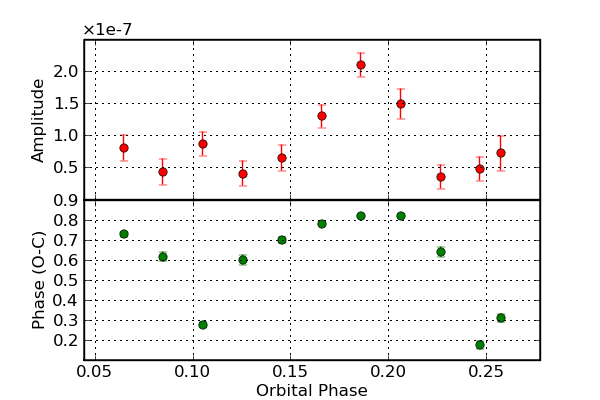
\includegraphics[bb=0 0 600 400,width=0.85\columnwidth]{images/archive_phot/S6670/S6670d_272.74.png}
 % S6544_23.13.png: 600x400 pixel, 100dpi, 15.24x10.16 cm, bb=0 0 600 400
 \caption[S6670 $O-C$ diagram of 272.74 s QPO]{Amplitude and $O-C$ variation of 272.74 s QPO of run S6670. Diagrams were calculated relative to a period of 272.74 s using 2 cycles with 50\% overlap. }
 \label{S6670_272.74}
\end{figure}

\pagebreak











